% !TEX root = ../../prj4projektdokumentation.tex
% SKAL STÅ I TOPPEN AF ALLE FILER FOR AT MASTER-filen KOMPILERES 

\section{Intern blok diagram}
På figur \ref{fig:IBDSp} og figur \ref{fig:IBDSt} ses IBD for henholdsvis Spændingsregulator og Styringsenhed. På diagrammerne ses de interne forbindelser i systemet. Under figurne er tilhørende signalbeskrivelser, se tabel \ref{tab:SignalbeskrivelseSp} og tabel \ref{tab:SignalbeskrivelseSt}, der uddyber diagrammerne nærmere.

\begin{figure}[htbp] % (alternativt [H])
	\centering
	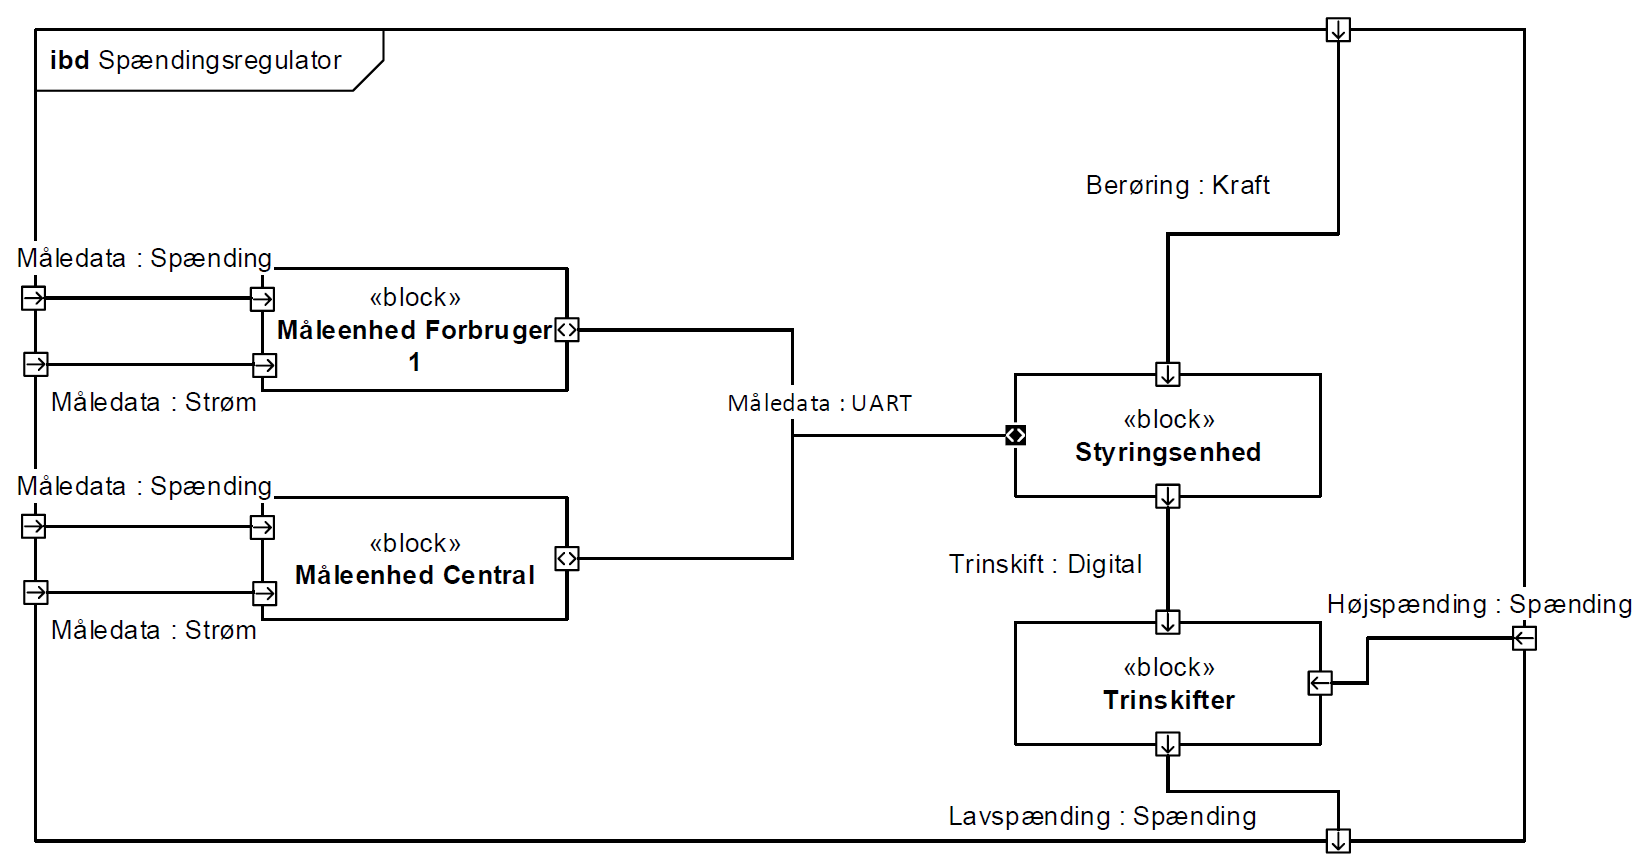
\includegraphics[width=0.8\textwidth]{Figure/IBDSpaendingsregulator1}
	\caption{IBD for Spændingsregulator}
	\label{fig:IBDSp}
\end{figure}

\begin{figure}[htbp] % (alternativt [H])
	\centering
	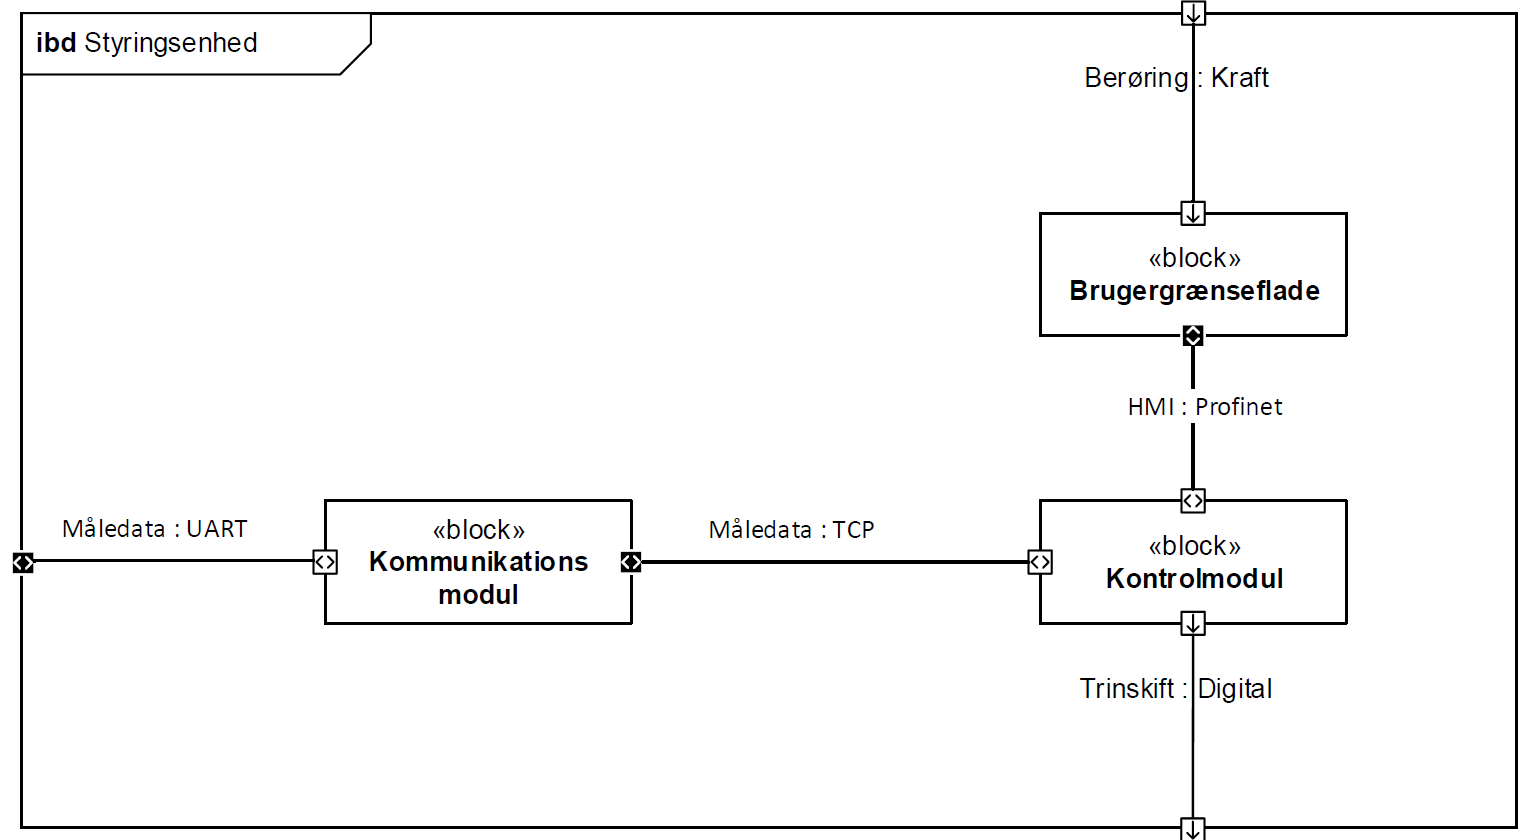
\includegraphics[width=0.8\textwidth]{Figure/IBDStyringsenhed1}
	\caption{IBD for Styringsenhed}
	\label{fig:IBDSt}
\end{figure}


\begin{table}[H]
	\centering
	\begin{tabular}{|l|l|l|l|p{4cm}|}
		\hline
		\textbf{Blok} & \textbf{Navn} & \textbf{Type} & \textbf{Signal} & 
		\textbf{Beskrivelse} \\\hline
		
		\multirow{3}{*}{Måleenhed} 
		& Måledata & Spænding & In & Måledata er spændingsniveauet på distributionslinjen. \\\hhline{~----} 
		& Måledata & Strøm & In & Måledata er strømniveauet på distributionslinjen. \\\hhline{~----} 
		& Måledata & UART & InOut & UART forbindelse til Styringsenhed \\\hline
		
		\multirow{3}{*}{Styringsenhed} 
		& Måledata & UART & Inout & UART forbindelse til Måleenhed \\\hhline{~----} 
		& Berøring & Kraft & In & Tryk på Brugergrænseflade \\\hhline{~----} 
		& Trinskift & Digital & Out & Trinskift er en digital kommando til Trinskifter \\\hline
	
		\multirow{3}{*}{Trinskifter} 
		& Trinskift & Digital & In & Trinskift er en digital kommando fra Styringsenhed. \\\hhline{~----} 
		& Højspænding & Spænding & In & Er spændingen på højspændingssiden af tranformeren. \\\hhline{~----} 
		& Lavspænding & Spænding & Out & Er spændingen på lavspændingssiden af transformeren. \\\hline
	\end{tabular}
	\caption{Signalbeskrivelse for Spændingsregulator}
	\label{tab:SignalbeskrivelseSp}
	
\end{table}

\begin{table}[H]
	\centering
	\begin{tabular}{|l|l|l|l|p{4cm}|}
		\hline
		\textbf{Blok} & \textbf{Navn} & \textbf{Type} & \textbf{Signal} & 
		\textbf{Beskrivelse} \\\hline
		
		\multirow{2}{*}{Brugergrænseflade} 
		& Berøring & Kraft & In & Tryk på Brugergrænseflade \\\hhline{~----} 
		& HMI & Profinet & InOut & Forbindelse til Kontrolmodul \\\hline
		
		\multirow{3}{*}{Kontrolmodul} 
		& HMI & Profinet & InOut & Forbindelse til Brugergrænseflade \\\hhline{~----} 
		& Trinskift & Digital & Out & Trinskift er en digital kommando til Trinskifter \\\hhline{~----} 
		& Måledata & TCP & InOut & TCP forbindelse til Kommunikationsmodul \\\hline
		
		\multirow{2}{*}{Kommunikationsmodul} 
		& Måledata & TCP & InOut & TCP forbindelse til Kontrolmodul \\\hhline{~----} 
		& Måledata & UART & InOut & UART forbindelse til Måleenhed \\\hline
	\end{tabular}
	\caption{Signalbeskrivelse for Styringsenhed}
	\label{tab:SignalbeskrivelseSt}
	
\end{table}


\newpage